Our baseline model is a U-Net~\cite{unet} model.
However, as opposed to the original U-Net paper, we do not crop the tensors in the skip connection.
Rather, we upsample the tensors from the lower depth to the size of the tensors in the skip connection through nearest-neighbours upsampling.
This is to preserve the size of the input image and generalize to image sizes that are not powers of 2.

At each U-Net depth, we use a block of two 2D convolution layers with residual connections~\cite{resnet} between the inputs and the block outputs.
Each 2D convolution layer is preceded by dropout~\cite{dropout} and succeeded by batch normalization~\cite{batch-norm} and then a leaky ReLU activation function.
If the number of channels changes, then the skip connection has a $1 \times 1$ 2D convolution layer to transform the channels in the inputs.
Otherwise the skip connection is an identity function.

Initially, the three RGB channels are transformed into $c_1$ channels.
At every depth, the number of channels increases by a factor of 2, until it reaches a fixed upper cap ($c_\mathrm{max}$).%chktex 35

Refer to Table~\ref{tab:unet-hyper-params} for further architecture specifics.
Refer to Figure~\ref{fig:arch} for the architecture diagram.

\begin{table}[h]
    \centering
    \caption{U-Net architecture hyper-parameters}%
    \label{tab:unet-hyper-params}
    \begin{tabular}{l r}
        \toprule
        Hyper-parameter & Value \\
        \midrule
        U-Net depth & 6 \\
        Dropout & 0.1 \\
        Initial channels ($c_1$) & 64 \\
        Maximum channels ($c_\mathrm{max}$) & 1024 \\%chktex 35
        2D convolution kernel size & $3 \times 3$ \\
        2D convolution padding & SAME \\
        Leaky ReLU slope & 0.2 \\
        Max pooling kernel size & $2 \times 2$ \\
        \bottomrule
    \end{tabular}
\end{table}

\begin{figure}
    \centering
    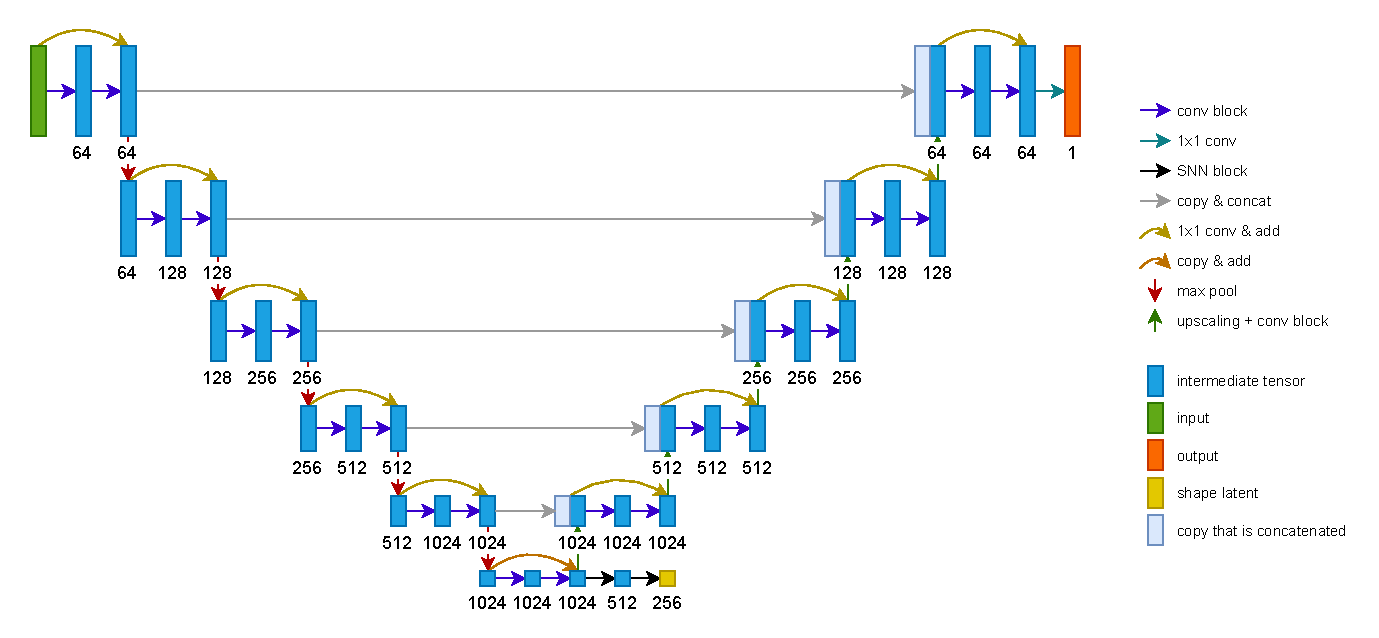
\includegraphics[width=0.9\textwidth]{images/CIL-arch.pdf}
    \caption{The model's architecture}%
    \label{fig:arch}
\end{figure}
